\hypertarget{theoretical-conceptual-foundations-and-state-of-the-art}{%
\section{Theoretical-Conceptual Foundations and State of the Art}\label{theoretical-conceptual-foundations-and-state-of-the-art}}

\subsection{1.1. Bedload transport as a multiphase environmental and engineering problem}

Sediment transport, defined as the solid particle's displacement within a fluid medium, governs river and coastal morphodynamics and directly affects the hydraulic efficiency of slurry and tailings transport in mining (\cite{PEND_Kaushal2002,PEND_Kaushal2012,PEND_Mesa2021,vreman__2015}). Bedload transport is especially critical, occurring within a thin near-bed layer only a few particle diameters thick where turbulence, gravity, particle inertia, and particle--bed contact interact most intensely, yet it can account for up to 60\% of total sediment load in gravel-bed rivers (\cite{garcia__2008,PEND_Nio1996,vanrijn__1984,PEND_Zhao2020}). Motion begins once flow shear stress exceeds the particles\textquotesingle{} critical threshold, proceeding via sliding, rolling, or saltation---the dominant mechanism at higher shear, governed by the balance of hydrodynamic and gravitational forces (\cite{garcia__2008,PEND_Hu1996,julien__2010,PEND_Lee1994,moreno-casas__2022,PEND_Nio1994,PEND_Nio1998}).

Beyond hydraulics, inaccurate bedload prediction compromises erosion, channel stability, and contaminant redistribution estimates, since particles also carry adsorbed pollutants affecting water quality (\cite{PEND_Bustamante2020,PEND_Gonzlez2008,walling__2006}). Industrially, poor prediction of settling and deposition in dense tailings flows drives wall erosion, operational shutdowns, and maintenance costs, while unaccounted flow relaminarization under heavy loading biases transport estimates (\cite{elghobashi__1994,gore__1989,PEND_Islam2024,PEND_Mesa2021,zhou__2020}).

Sediment transport has traditionally relied on empirical formulations valued for simplicity (\cite{vanrijn__1984,yalin__1977}). The Meyer-Peter and Müller \cite{meyer-peter__1948} equation remains a classical reference expressing dimensionless transport rate as a function of shear stress, but its predictive capability is restricted to its calibration conditions and it neglects microscale turbulent stresses and the stochastic, coherent-structure-driven nature of entrainment (\cite{ancey__2020,PEND_Lee1994,PEND_Wiberg1985}). Einstein\textquotesingle s \cite{einstein__1950} statistical framework similarly relates transport to entrainment probability but still assumes homogeneous, time-invariant behavior (\cite{ancey__2020,PEND_Furbish2016}). Neither resolves the near-wall sweep and ejection events (Q4/Q2) that physically control entrainment intermittency (\cite{PEND_Baker2021,PEND_Nio1994,PEND_Nio1996,PEND_Nio1998,zhou__2020}), explaining deviations of two to six orders of magnitude from measured rates (\cite{ancey__2020,chassagne__2020,wong__2006}), bedload being fundamentally a stochastic, multiphase problem governed by microscale fluid--particle and particle--particle interactions (\cite{balachandar__2010,PEND_Chen2024,PEND_Schmeeckle2014,yamamoto__2001}).

These limitations get worse by increasing local concentration. Once the solid volume fraction \(\phi_{v}\) exceeds \(10^{- 3}\) (0.1\%), the system exits mean shear/entrainment threshold control and enters a four-way coupling regime, governed by coupled interactions among turbulence, hindered settling, interparticle collisions, and concentration-dependent hydrodynamic forces such as non-linear drag, Saffman lift, and Basset history force (\cite{balachandar__2010,elghobashi__1994,PEND_Elghobashi2006,PEND_Mesa2021,moreno-casas__2022}). Frictional contacts and collective effects introduce dispersive stresses and modify effective viscosity and mixture density---a granular rheology (µ(I) rheology, kinetic theory of granular flows) that renders empirical equations fundamentally insufficient for dense transport (\cite{ancey__2020,chassagne__2020,PEND_Nio1994}).

This has driven a shift toward mechanistic frameworks centered on turbulence modulation: how particles reshape the fluid\textquotesingle s TKE budget depending on Stokes number, mass loading, and density ratio (\cite{capecelatro__2013,PEND_Crowe2012,gao__2023}). Small heavy particles in dilute suspensions attenuate TKE via turbophoresis and suppressed quasi-streamwise vortices, while high-inertia particles or dense clusters enhance production through wake shedding (\(Re_{p} < 400\)) and boundary collisions (\cite{PEND_Brandt2021,brandt__2022,elghobashi__1994,PEND_Elghobashi2006,PEND_Lee2015,PEND_Liu2022}), an effect that is highly non-monotonic with mass loading, acting as sink or source depending on concentration, and directly impacting sediment suspension capacity and bed force balance (\cite{guta__2024,zhou__2020}).

Eulerian--Lagrangian CFD-DEM has become central to resolving these phenomena, coupling resolved fluid hydrodynamics (DNS/RANS/LES) with particle tracking via Newton\textquotesingle s second law (\cite{capecelatro__2013,moreno-casas__2022,PEND_Vreman2008}), ranging from unresolved point-particle methods with semi-empirical drag laws (\cite{PEND_Blais2016,PEND_Jaiswal2022}) to fully resolved PR-DNS capturing exact boundary-layer deformation via immersed boundary methods (\cite{brandt__2022,PEND_Mesa2021}), with hybrid semi-resolved approaches bridging the cost gap for dense bedload layers (\cite{PEND_Chen2024,PEND_Xu2025}).

Despite these advances, recent reviews conclude no single framework satisfactorily spans the full concentration range, from dilute suspensions to non-dilute frictional bedload transport (\cite{guta__2024,PEND_Li2020,zhou__2020})---motivating a shift toward the microscale fluid--discrete-phase interplay. The continuous phase develops vortical structures governing near-wall TKE redistribution (\cite{PEND_Nezu1993,PEND_Pope2000}), while particles either remain suspended, modifying the velocity profile, or migrate toward the bed via turbophoresis depending on their Stokes and Reynolds numbers (\cite{PEND_Bassenne2018,PEND_Elghobashi2006,nezu__2004}). Near the bed, particle dynamics transition from hydrodynamic suspension to a regime dominated by frictional contacts and inelastic collisions (\cite{maurin__2017,PEND_Doren2023}), setting the stage for the physical classification of particle-laden flow regimes.

\subsection{1.2. Physical Classification of Particle-Laden Flows: From Dilute to Non-Dilute Four-Way Coupling}

Particle-laden flow dynamics are fundamentally governed by the solid volume fraction (\(\phi\)), which dictates both the macroscopic flow regime and the physical mechanisms required to model the momentum exchange between phases. Distinction between the dilute and non-dilute regime is traditionally classified through the established framework by Elghobashi \cite{elghobashi__1994,PEND_Elghobashi2006}.

In dilute regimes (typically \(\Phi \leq 10^{- 6}\)) (\cite{elghobashi__1994}), the distance between particles is large enough that interparticle collisions are negligible. The flow is characterized by one-way coupling, where the fluid fully dictates particle motion via hydrodynamic forces, but particles are dynamically "invisible" to the carrier fluid's turbulence (\cite{elghobashi__1994,PEND_Elghobashi2006,balachandar__2010,messa__2021}). As the volume fraction increases into the transitional dilute regime (\(10^{- 6} < \Phi \leq 10^{- 3}\)), the mass loading becomes comparable to the carrier phase, and the system enters a two-way coupling state. The influence of the dispersed phase modulates the fluid\textquotesingle s turbulent kinetic energy (TKE) by generating viscous dissipation of sub-grid eddies, depending on the particle Stokes number (\(St\)) and the particle to eddy size ratio (\cite{balachandar__2010,hu__2025,PEND_Li2025,PEND_Liu2022}).

However, as the concentration increases through the critical threshold (\(\Phi > 10^{- 3}\)), the flow transitions into the non-dilute or dense regime. In this state, the assumptions of isolated hydrodynamics break down, making four-way coupling a strict physical requirement rather than a mere numerical refinement (\cite{messa__2021,vreman__2015}). The dense regime is characterized by the dominance of particle-particle interactions, collisional momentum redistribution, and collective structural rearrangement (agglomeration and break-up). At extreme concentrations, the granular flow sub-regime emerges, where interparticle collisions and enduring frictional contacts govern the stress tensor, rendering the interstitial fluid dynamics a secondary, albeit modifying, factor (\cite{maurin__2017,zhao__2023}).

\subsection{1.3. Turbulence modulation in non-dilute open-channel flow}

\subsubsection{1.3.1. Early criteria for attenuation and enhancement}

The microphysics of turbulence modulation in the four-way coupled regime are different from the two-way regime. In dilute suspensions, particles with low momentum numbers tend to attenuate turbulence by dragging fluid eddies, while larger particles (\(St > 1\)) enhance it through wake shedding (\cite{balachandar__2010,PEND_Liu2022}). Conversely, in dense suspensions, attenuation is overwhelmingly dominant due to combined hydrodynamic and collisional mechanisms.

Turbulence attenuation or enhancement depends intrinsically on particle size, inertia, and concentration (\cite{PEND_Li2025,motoori__2024,PEND_Rohilla2023}). Gore and Crowe \cite{gore__1989} proposed a foundational size-based criterion linking turbulence modulation to the ratio between particle diameter and the turbulent integral scale, predicting that particles smaller than 0.1 times the integral scale attenuate turbulence, whereas larger particles enhance it through wake-induced production (\cite{motoori__2024,nezu__2004,PEND_Rohilla2023,vreman__2015}). Later, Kulick et al. \cite{kulick__1994} demonstrated experimentally that turbulence attenuation increases monotonically with both Stokes number and mass loading, and that this attenuation is inherently anisotropic, affecting spanwise and wall-normal velocity fluctuations more severely than streamwise ones (\cite{PEND_Vreman2007,yamamoto__2001}). In addition, Pan and Banerjee \cite{pan__1996} showed through two-way coupled DNS in channel flows that particles smaller than the Kolmogorov dissipative scale tend to suppress turbulent fluctuations, whereas larger particles may enhance them (\cite{baker__2019,PEND_Shao2012,PEND_Wang2020,yamamoto__2001}).

However, recent multiphase flow studies explicitly caution that these dimensionless criteria were established primarily in homogeneous dilute to moderate regimes. Consequently, they remain unvalidated or exhibit entirely different governing mechanics, when applied to the dense near bed regime of open channels, where granular friction, high volume fractions, and four-way coupling dominate (\cite{capecelatro__2018,chauchat__2017,PEND_Innocenti2021}).

\subsubsection{1.3.2. Concentration-dependent turbulence modulation}

Particle concentration modifies turbulence not only locally but across multiple scales and flow topologies. In point-particle Eulerian-Lagrangian DNS and Lagrangian PDF models, increasing mass loading produces a systematic reduction in turbulent kinetic energy (TKE) (\cite{capecelatro__2018,PEND_Innocenti2021,PEND_Zhao2013}). Moreover, two-way particle feedback significantly alters momentum coupling by damping wall-normal velocity fluctuations, which consequently reduces \emph{turbophoresis} (physical tendency of suspended heavy particles to drift away from high-intensity turbulence towards calmer regions) (\cite{PEND_Bassenne2018,PEND_Lee2019,PEND_Sardina2012,PEND_Zahtila2023}).

Simultaneously, concentration effects are not universally monotonic and depend significantly on domain scale and local turbulent structures. Through high Reynolds number point-particle DNS in open channel flow, Gao et al. \cite{gao__2023} found that both large-scale motions (LSMs) and very-large-scale motions (VLSMs) weaken under particle loading, contrasting with the VLSM enhancement observed at more moderate Reynolds numbers. Furthermore, Hassaini and Coletti \cite{hassaini__2022} showed experimentally that settling particles may enhance turbulence at small scales by injecting gravitational potential energy into the flow, overcoming the attenuation typically associated with high mass loading in zero-gravity environments (\cite{brandt__2022,chouippe__2023}). These results demonstrate that concentration modifies turbulence in a highly coupled and scale-dependent manner, thereby altering the physical conditions and velocity spectra that governs settling, suspension, and bedload transitions (\cite{capecelatro__2018,gao__2023,PEND_Zhao2013}).

\subsubsection{1.3.3. Implications for the Turbulent Kinetic Energy budget}

The TKE budget departs significantly from its single-phase form in particle-laden flow. Beyond mean-shear production, transport, and viscous dissipation, an interphase feedback term acts as a local source or sink of fluid TKE depending on particle inertia, slip velocity, concentration, and position across the flow; in sediment-laden channels this budget must further account for density-stratification effects that alter the production--transport--dissipation balance (\cite{brandt__2022,capecelatro__2018,gualtieri__2023,guta__2024,vreman__2015,PEND_Zhao2013}). This feedback cannot be represented by a single universal sink term: at low mass loading, mean-shear production dominates; at intermediate loading, relaminarization may occur; and at high loading, turbulence is instead generated predominantly by mean interphase slip ("drag production") (\cite{capecelatro__2018,gualtieri__2023}). Particle feedback can thus severely reduce turbulence production and transport while simultaneously modifying dissipation and interphase-exchange terms (\cite{vreman__2015,zhou__2020})---meaning a reduction in bulk TKE does not imply that every local energy pathway is equally weakened.

Two mechanisms explain why point-particle descriptions fail to capture this budget in the non-dilute regime. (i) Finite-size effects: particle surfaces impose no-slip conditions and distort nearby eddies, locally intensifying velocity gradients and producing dissipation up to three times higher in the immediate particle vicinity, while particle wakes generate TKE via vortex shedding at sufficiently large particle Reynolds numbers even as they simultaneously drain energy toward dissipation-range motions, starving the larger energy-containing scales (\cite{balachandar__2010,brandt__2022,capecelatro__2018,PEND_Finn2016,guta__2024,zhang__2025,PEND_Zhao2013}). (ii) Collision-mediated pathways: within the granular phase, energy partitions into correlated mean motion and uncorrelated fluctuations (granular temperature), and because interparticle collisions are inherently inelastic, they act as a massive thermodynamic sink that must be continuously replenished by drag extraction from the fluid, accelerating fluid TKE dissipation (\cite{afkhami__2015,capecelatro__2018,chauchat__2017,vreman__2015}). Depending on collision properties and local concentration, this can suppress near-wall accumulation or generate localized ejections and sweeps, disrupt large-scale coherent wall vortices, attenuate streamwise vortex energy, and induce anisotropy that inhibits energy redistribution into wall-normal and spanwise motions; with DNS confirming that collisions flatten the mean particle velocity profile by transferring kinetic energy from streamwise into normal fluctuations (\cite{hu__2025,PEND_Lee2015,PEND_Liu2022,nasr__2009,ven__2024,vreman__2015}).

A further distinct contribution comes from pseudo-turbulence: fluctuations arising from the superposition of particle-induced disturbance flows and wakes, concentrated over particle-scale lengths, which generate strongly anisotropic Reynolds stresses distinct from shear-produced turbulence. In sediment-laden boundary layers, their interaction with near-bed coherent structures can shift the TKE-production peak upward toward the top of the bedload layer, driving enhanced downward TKE transport into the sediment-rich region (\cite{brandt__2022,guta__2024,moore__2019}).

The closure of the TKE budget therefore remains the central modeling challenge for dense sediment transport. The unresolved coupling among concentration, interphase slip, wakes, inelastic collisions, stratification, and coherent turbulent structures directly motivates the need for microscale, four-way coupled frameworks.

\subsection{1.4. Hindered-settling and quasi-steady drag closures}

\subsubsection{1.4.1. Classical hydrodynamic force formulations}

Individual rigid-sphere motion in Eulerian-Lagrangian models is commonly formulated through the Maxey-Riley-Gatignol framework (\cite{PEND_Gatignol1983,maxey__1983}), balancing buoyancy, quasi-steady drag, pressure-gradient, added mass, and Basset history forces, with lift sometimes added for sheared flows (\cite{balachandar__2010,brandt__2022}). Its value lies in separating instantaneous hydrodynamic effects from the memory of prior relative acceleration, captured by the Basset term (\cite{PEND_Crowe2012,PEND_Prosperetti2007}).

This is not a general dense-suspension theory: it requires vanishing particle Reynolds number, diameters much smaller than the Kolmogorov scale, and dilute conditions where interparticle interactions are negligible (\cite{balachandar__2010,elghobashi__1994,kuerten__2016})---assumptions especially restrictive near the bed, where particle size approaches turbulent scales and particle-particle/wall interactions become important (\cite{messa__2021,PEND_Shao2012}). Term importance also depends on density ratio: in liquid-solid systems, added mass, pressure-gradient, and history effects can become significant near the Kolmogorov scale (\cite{kuerten__2016,PEND_Rupp2023}), so neglecting them requires case-specific justification rather than universal simplification.

In practice, most simulations instead rely on quasi-steady drag closures---Schiller-Naumann \cite{PEND_SchillerNaumann1935}, Wen-Yu \cite{PEND_WenYu1966}, or Gidaspow-type formulations---parameterizing force through particle Reynolds number, slip velocity, and volume fraction; efficient for dilute conditions but highly uncertain in non-dilute, clustered, turbulence-modulated suspensions, since real flows contain concentration gradients, wakes, and wall effects that mean-drag closures cannot capture (\cite{PEND_Gualtieri2014,willen__2019}). Particle clusters, for instance, can experience lower total drag than well-separated particles due to wake interference, while rising volume fractions promote collisions that disrupt clusters and alter the instantaneous force balance (\cite{chouippe__2023,willen__2019}).

Conventional closures thus remain valid only as first-order dilute approximations; their use in dense, stratified flows requires validation against particle-resolved simulations, since the open problem is not the magnitude of mean drag but its dependence on local microstructure, fluctuating slip, and wall proximity (\cite{capecelatro__2013,osnes__2025}).

\subsubsection{1.4.2. Drag closures and force variance}

Classical closures relied on empirical single-particle expressions calibrated for dilute domains, such as Yen\textquotesingle s \cite{PEND_Yen1992} correlation used in stochastic saltation models (\cite{PEND_Nio1994,PEND_Nio1996}), ignoring solid volume fraction and wake interference---failing as inter-particle distances shrink in the non-dilute regime.

PR-DNS has shown that dense-suspension drag depends on structural factors absent from quasi-steady closures (\cite{brandt__2022,chouippe__2023}). The Tenneti-Garg-Subramaniam correlation (\cite{tenneti__2011}), derived from PR-DNS of fixed spherical assemblies, captures the joint influence of particle Reynolds number and local volume fraction by resolving hydrodynamic hindrance and wake interactions (\cite{capecelatro__2018,guta__2024}), with machine learning models more recently extending these datasets (\cite{PEND_He2019,PEND_Jiang2021}).

However, drag in freely evolving suspensions departs systematically from fixed-bed correlations, as particle mobility and clustering actively reorganize the flow and alter mean slip (\cite{tavanashad__2021,PEND_Doren2023})---making the force balance deeply concentration-, turbulence-, and fluctuation-dependent (\cite{brandt__2022,zhou__2020}).

A key advance is recognizing that dense suspensions require modeling drag variance, not just its mean, since point-particle methods using locally averaged fluid properties underpredict particle velocity variance (\cite{brandt__2022,moore__2019}). Stochastic closures address this, such as Lattanzi et al.\textquotesingle s \cite{lattanzi__2021} Langevin approach treating neighbor-induced drag fluctuations as an Ornstein-Uhlenbeck process fitted to PR-DNS data (\cite{osnes__2025}).

Critical gaps remain for near-wall flows: most closures assume spherical particles and uniform flow, whereas boundary shear induces asymmetric wakes and lift forces (\cite{PEND_Costa2020,PEND_Costa2021}), and irregular sediment morphology alters vorticity and force variance relative to ideal spheres (\cite{sanjeevi__2022,PEND_Zhao2024}). Extending variance-aware drag models to sheared boundary layers and non-spherical particles remains a primary open challenge.

\subsection{1.5. Particle-based simulation frameworks for microscale interaction analysis}

\subsubsection{1.5.1. Point-particle Eulerian-Lagrangian models}

Point-particle Eulerian-Lagrangian (PP-EL) models remain widely used for tracking large particle populations at low cost, advancing particles in a Lagrangian frame while solving the carrier fluid on an Eulerian grid, with fluid forces from empirical closures and reaction forces redistributed as a momentum source (\cite{messa__2021,PEND_Shao2012,PEND_Zhang2023}), well suited to parametric studies across Reynolds number, Stokes number, density ratio, and coupling level (\cite{PEND_Vreman2007,vreman__2015,zhou__2020}).

Formal validity, however, requires particle diameter much smaller than both the Kolmogorov scale and the local grid cell size \(\Delta_{c}(\Lambda = d_{p}/\Delta_{c} \ll 1)\ \)at low particle Reynolds number (\cite{balachandar__2010,elghobashi__1994,horwitz__2016,PEND_Horwitz2018}). Beyond this bound, the undisturbed fluid velocity cannot be properly defined at the particle position, producing unphysical feedback instabilities (\cite{horwitz__2016})---a critical issue near the bed, where the fine grid resolution needed to capture velocity gradients (typically paired with the WALE subgrid model for its near-wall behavior; \cite{PEND_Nicaud1999}) almost invariably pushes Λ≳1 for finite-sized sediment grains, violating the point-particle assumption.

Semi-resolved schemes avoid this---without the cost of fully resolved models---using fixed-width smoothing kernels to decouple momentum transfer from grid size (\cite{che__2024,PEND_Deb2013}). This regularization, however, creates a blind spot: since WALE depends only on resolved strain/rotation invariants, smoothing the particle feedback erases finite-size microscopic gradients, leaving the closure blind to near-field wake interactions and pseudo-turbulence, and underpredicting particle-induced dissipation by ignoring the thermodynamic sink of granular collisions (\cite{PEND_Crowe2012,PEND_Finn2016,moore__2019,vreman__2015}). PP-EL and standard semi-resolved methods must therefore be treated as reduced-order models requiring advanced subgrid closures, not fully predictive microscale representations (\cite{messa__2021,PEND_Rupp2023}).

Advanced formulations replace WALE with a transport equation for subgrid TKE (\(k_{sgs}\)), retaining temporal memory and including a two-way coupling source term (\(S_{k}\)) for the mechanical work of fluctuating drag, acting as an energy sink in dense suspensions (\cite{balachandar__2010,capecelatro__2018}). Since semi-resolved solvers cannot compute this dissipation ab initio, PR-DNS of representative control volumes is increasingly used as a "numerical laboratory" to calibrate \(S_{k}\) in macroscopic LES-DEM frameworks (\cite{chouippe__2023,PEND_Finn2016,tenneti__2011}).

\subsubsection{1.5.2. Particle-resolved DNS}

Particle-resolved DNS (PR-DNS) is the highest-fidelity framework for fluid-particle interactions, solving Navier-Stokes alongside rigid-particle motion on a mesh significantly finer than the particle diameter, resolving exact local velocity and pressure fields rather than point-force approximations (\cite{balachandar__2010,chouippe__2023,messa__2021}). The Immersed Boundary Method (IBM) is a widely used implementation, enforcing no-slip at the particle surface via momentum-exchange forcing without body-fitted remeshing; Lattice-Boltzmann moving-boundary methods offer a robust alternative (\cite{PEND_Crowe2012,PEND_Jin2016,PEND_Shao2012}).

By explicitly resolving the particle boundary layer and wake, PR-DNS provides first-principles estimates of drag, lift, surface-induced velocity gradients, local Reynolds stresses, and pseudo-turbulent fluctuations, capturing the mutual modification of neighboring wakes and near-field hindrance unavailable to point-particle laws (\cite{chouippe__2023,PEND_Crowe2012,moore__2019}). It is particularly valuable for finite-size effects: particles comparable to the smallest turbulent scales act as localized dissipation mechanisms, altering fluid volumes much larger than themselves (\cite{chouippe__2023,PEND_Finn2016,vreman__2015}). In wall-bounded flows, PR-DNS reveals configuration effects inaccessible to conventional models---preferential accumulation and sediment patterns (\cite{PEND_Kidanemariam2014}), scaling laws for dense suspensions (\cite{PEND_Costa2015}), and the exact non-monotonic feedback of finite-size particles on the turbulence spectrum (\cite{chouippe__2023,PEND_Picano2015})---making it the principal framework for generating drag, force-variance, and pseudo-turbulence closures for macroscopic models (\cite{kuerten__2016,moore__2019,tavanashad__2021}).

Its paramount limitation is computational cost: resolving near-field flow requires roughly ten or more grid cells across a particle diameter, and realistic sediment-transport patterns may demand up to 10¹⁰ grid nodes, 10⁵--10⁷ grains, and integration times of at least 10³ bulk time units (\cite{elghannay__2018,rupp__2021}). PR-DNS studies of open-channel transport thus remain heavily restricted in particle count, domain size, Reynolds number, and duration (\cite{elghannay__2018,PEND_Jaiswal2022,vreman__2015})---positioning PR-DNS not as an engineering-scale predictive tool, but as a fundamental "numerical laboratory" for generating the closures needed to model dense sheet-flow transport in computationally tractable frameworks.

\subsection{1.6. Optical measurement techniques for particle-laden validation}

\subsubsection{1.6.1. Experimental validation as a constraint on model development}

Progress in modeling dense sediment transport is constrained not only by incomplete closures but by the scarcity of validation datasets resolving velocity, concentration, and turbulence in the near-bed region at compatible scales (\cite{elghannay__2018}). Earlier sheet-flow experiments relied on intrusive pointwise probes yielding non-collocated, one-component measurements (\cite{PEND_Donoghue2004,revil-baudard__2015,PEND_Sumer1996}), while later video-based approaches provided two-component velocities and concentration profiles but were largely confined to the sidewall, suffering boundary effects (\cite{PEND_Capart2011,PEND_Lajeunesse2010,PEND_Spinewine2011}). Simultaneously resolving the turbulent flow field and all sediment particle motion remains a profound experimental challenge, despite being necessary to link coherent structures to entrainment (\cite{PEND_Cellino2004,PEND_Nio1996,revil-baudard__2015}).

Within this context, the sheet-flow dataset of Revil-Baudard et al. \cite{revil-baudard__2015} stands as a key reference: using Acoustic Concentration and Velocity Profiling (ACVP), they obtained collocated bed-normal profiles of streamwise/wall-normal velocity, solid concentration, and sediment flux across both bedload and suspension layers, supporting subsequent TKE-budget research (\cite{PEND_Fromant2019,guta__2024}). This dataset does not eliminate uncertainty in the dense transition region, however---acoustic concentration estimates carry statistical biases and near-bed interface detection remains difficult (\cite{revil-baudard__2015,PEND_Thorne2014}). Critically, the measured wall-normal velocity in high-inertia ACVP represents a mixture velocity rather than the isolated sediment-phase velocity, undermining vertical flux accuracy (\cite{guta__2024}); modern closures instead require phase-resolved covariance data, such as concentration fluctuations from Acoustic Particle Flux Profiling (\cite{PEND_Cellino2004}), rather than mere bulk-profile agreement (\cite{PEND_Toorman2003}).

This gap is reflected in modeling itself: in SedFoam-2.0, neither tested granular-stress model recovered the measured concentration in the densest sheet-flow layer, while velocity profiles proved highly sensitive to turbulence-model calibration (\cite{chauchat__2017,maurin__2016}). Disagreement in this region thus reflects the coupled difficulty of measuring and modeling concentrated granular layers governed by contact, collision, and turbulence modulation---not model failure or measurement bias alone.

\subsubsection{1.6.2. Optical techniques}

Non-intrusive optical techniques remain indispensable for spatially distributed flow information without probe-induced disturbance. Particle Image Velocimetry (PIV) quantifies velocity fluctuations, Reynolds stresses, and coherent structures, while combined PIV/PTV enables phase discrimination between fluid tracers and sediment (\cite{PEND_Adrian1991,PEND_Nezu2011,raffel__2018}). The two are complementary: PIV yields an Eulerian field via cross-correlation of particle-image ensembles, while PTV tracks individual particles for Lagrangian trajectories (\cite{PEND_Khler2012})---critical in sediment-laden flows, since inertial particles can exhibit uncorrelated velocities or trajectory crossings that only PTV captures (\cite{PEND_Ouellette2006}).

Standard optical velocimetry is limited by a strict trade-off between image density and particle identifiability: higher concentration improves PIV correlation but causes occlusion and spurious vectors (\cite{PEND_Scharnowski2020}), while PTV requires sparse images to track identities unambiguously, failing under dense clustering (\cite{PEND_Khler2012}). Without index matching, dense-layer measurements are thus restricted to 2D monolayers or sidewall-adjacent particles (\cite{PEND_Frey2014,ni__2018}).

Refractive-Index Matching (RIM) extends optical access into dense suspensions using particles and fluids of matched refractive index (\cite{PEND_Dijksman2012,PEND_Wiederseiner2011}), though it is highly sensitive to temperature and chemical impurities (\cite{PEND_Wiederseiner2011}). Tuned RIM experiments have nonetheless achieved breakthroughs---Baker \& Coletti \cite{baker__2019} resolved boundary-layer turbulence up to 25\% solid volume fraction using hydrogel spheres, and matched-index scanning has extracted Reynolds stresses, granular temperature, and interphase drag in 3D mobile beds (\cite{ni__2018}). RIM\textquotesingle s overriding limitation remains representativeness: surrogate particle material, density ratio, friction, and restitution must stay physically relevant to real sediment-water dynamics.

\subsubsection{1.6.3. Dense-layer validation gap}

Despite advancements in both acoustic and optical diagnostics, a severe experimental validation gap persists in the volume fraction range of \(\phi_{v} \approx 0.30 - 0.50\), which physically characterizes the dense sheet-flow bed layer. Acoustic methods lose phase-resolved accuracy due to signal saturation and multiple scattering, optical methods lose penetration depth due to opacity and image overlap, and electromagnetic methods currently lack the required spatial and temporal resolution for turbulence. While emerging techniques such as MRI velocimetry, X-ray CT, and tomographic PTV represent promising future directions, they are not yet standard tools capable of fully resolving simultaneous fluid-solid turbulence in dense mobile beds. Consequently, the reliance on high-fidelity, particle-resolved computational frameworks (PR-DNS) is no longer just a numerical exercise, but an absolute necessity to bridge the dense-layer validation gap and generate the closures required for macroscopic engineering models.

\hypertarget{hypothesis-and-goals}{%
\section{Hypothesis and Goals}\label{hypothesis-and-goals}}

Particle concentration in non-dilute open-channel flow does not merely alter sediment transport through hindered settling; rather, it actively modulates fluid turbulence, modifies the turbulent kinetic energy budget, and changes the effective hydrodynamic force balance acting on particles. Conventional hindered-settling relations and quasi-steady drag closures are inadequate because they do not incorporate concentration-dependent turbulence modulation, neighbor induced force fluctuations, pseudo-turbulent production, and collisional redistribution of energy. Dense regime requires four-way coupling due to particle-particle interactions that qualitatively modify both fluid and particle dynamics. Although particle-based simulation frameworks provide the most promising path toward a physically interpretable description of microscale interaction mechanisms, their development remains constrained by closure deficiencies and by the lack of fully reliable validation data in the dense near-bed region.

This research addresses the study of microscale physics of turbulent sediment-laden flow across the dilute and non-dilute concentration regime in an open channel flow. The study considers a single type of spherical particle of diameter \(0.70\ mm\), with particle Reynolds number, \(Re_{p} = 73\), Stokes number, \(St \approx 1.79\), and Shields parameter, \(\theta \approx 0.043\), with the presence of a bedload transport condition. Particle volume fractions range from the dilute \((\phi < 0.1\%)\) to the non-dilute regime \((\phi \geq 0.1\%)\), where four-way coupling effects are expected to become dominant, with an initial flow Reynolds number, \(Re \approx 10,000\).

Following the former information, this proposal relies on the following research question and hypothesis:

\textbf{Research question:} How does increasing particle concentration to the non-dilute regime, at \(\mathbf{St} \sim \mathbf{O}(\mathbf{1})\), modify turbulence structure and effective hydrodynamic force balance in open-channel flows? Can a four-way coupled computational model framework, validated with non-intrusive techniques, accurately capture the microscale physics of multiphasic interaction to propose simplified equations that improve the estimation of bedload transport rate?

\emph{\textbf{Hypothesis}}

\emph{Turbulence modulation is governed primarily by the particle-fluid momentum feedback and interparticle collisions, such that: (i) streamwise turbulence intensity,} \(u_{rms}^{'}\)\emph{, attenuation increases monotonically with solid volume fraction,} \(\phi_{v}\)\emph{, at fixed friction velocity,} \(u_{\tau}\)\emph{, only captured by a four-way coupled model, (ii) turbulence attenuation rate with respect to} \(\phi_{v}\) \emph{reaches a maximum near} \(St^{+} \approx 5\)\emph{, consistent with the preferential concentration mechanism, and, (iii) for} \(u_{\tau} > 4\ cm/s\)\emph{, inter-particle collisions become the dominant momentum exchange mechanism, in the non-dilute bedload transport regime of granular sediments (}\(d_{p} = 0.7\ mm,\rho_{p}/\rho_{f} = 2.65\)\emph{) in turbulent open-channel flow at} \(Re \sim 10⁴\)\emph{, where the solid volume fraction exceeds the four-way coupling threshold (}\(\phi_{v} > 10⁻³\)\emph{) and the friction velocity lies in the} \(u_{\tau} \in \lbrack 1,\ 3\rbrack\ cm/s\) \emph{range.}

\textbf{General Goal}

To develop a four-way coupling CFD-DEM turbulent model for open-channel flow, \(Re \sim 10^{4}\), capable of predicting how particle concentration modifies turbulence structure and particle hydrodynamic interactions, experimentally validated with non-intrusive optical techniques across the dilute and non-dilute particle concentration per volume fraction regime, to understand the microscale particle physic behavior in \(St^{+} \sim O(1)\) regime with the aim of proposing simplified equations to enhance the bedload sediment transport estimation.

The specific objectives (SO) of the proposal correspond to the following:

\textbf{SO1:} To develop an Eulerian model (CFD) in OpenFOAM, that incorporates a dynamic SGS model incorporating calibrated non-linear drag closure equation and particle concentration feedback, coupled in four-ways with an \emph{in-house} GPU Lagrangian tracking model (DEM) code to simulate multiphasic interaction, wall-particle and particle-particle collisions, that validate the individual particle dynamics according to the saltation trajectories given by Niño \& García, 1998.

\textbf{SO2:} To experimentally characterize the CFD-DEM model, using granular sediments of 0.7 mm diameter, friction velocities, \(u_{\tau},\) in the range of \(\lbrack 1,\ 3\rbrack\ cm/s\) and particle concentration per volume fraction from the non-dilute range up to the maximum optically visible concentration, \(\phi \in \lbrack 10^{- 3}\ ,\ \phi_{\max,opt}\rbrack\), simultaneously acquiring PIV and PTV measurements of the continuous and discrete phase, respectively, throughout the optically accessible concentration range.

\textbf{SO3:} To validate the CFD-DEM with respect to the experimental data, using time-average velocity profiles, turbulence intensity statistics, \((u_{rms}^{'},v_{rms}^{'})\), with a maximum error of 15\% and particle velocity distributions with a maximum error of 20\%, throughout space.

\textbf{SO4:} To quantify the Turbulent Kinetic Energy (TKE) balance behavior given by the particles as a function of concentration and Stokes number in wall units and identify the transition between two-way and four-way coupling regime under the same flow conditions.

\textbf{SO5:} To extrapolate the validated model on the optic limit to characterize the rheological behavior of the multiphase mixture as the particle concentration increases and identify the onset of the Bagnold inertial regime.

\hypertarget{scientific-or-technological-novelty}{%
\section{Scientific or technological novelty}\label{scientific-or-technological-novelty}}

This proposal introduces a physics-based, multiscale framework to understand and predict the mechanisms governing turbulence modulation in open-channel flows, through three linked contributions. The \underline{first} innovation is the use of a four-way coupled, unresolved/\textbf{semi-resolved (by the kernels implementation)} CFD-DEM model that incorporates momentum transfer and fluid-particle interaction forces within the WALE subgrid-scale closure of LES, aiming to predict how particle concentration modulates carrier-fluid turbulence in the non-dilute regime. In its standard form, the WALE sub-model does not correctly transfer the effect of particle motion and collisions onto the unresolved scales, limiting its physical accuracy in this regime. The \underline{second} contribution is the development of a resolved DNS model on a smaller-scale domain, capable of fully resolving the turbulence field around particles and benchmarking against LES results. This data will inform a modified WALE closure that explicitly incorporates particle effects on unresolved scales. Existing fluid-particle coupling instead relies on empirical force models (drag, lift, virtual mass) derived under restrictive dilute-regime assumptions: isolated, rigid, spherical particles smaller than the Kolmogorov scale, at low particle Reynolds number, in an undisturbed velocity field. These assumptions remain systematically unvalidated in the non-dilute regime, where collisions and forces induced by neighbor force fluctuations are no longer negligible. The proposed approach is thus expected to yield physically consistent predictions of turbulence dynamics as a function of particle concentration. The \underline{third} contribution is an experimental validation methodology combining simultaneous PIV and PTV to quantify both fluid velocity and particle motion at non-dilute concentrations (volume fractions above 0.1\%). Together, these three contributions provide an experimentally validated advance in describing particle-induced turbulence modulation, extending current understanding of the non-dilute regime and enabling calibrated expressions for dimensionless sediment transport.

\hypertarget{methodology}{%
\section{Methodology}\label{methodology}}

The proposed methodology for this research encompasses both numerical simulations and experimental approaches (see Figure 4.1). The first stage consists of microscale calibration using PR-DNS models. The second stage involves the computational modeling of a turbulent open-channel flow to understand the microscale physical interaction with varying volume fraction concentrations of homogeneous granular sediment particles. This is analyzed in terms of hydrodynamics, momentum transfer, and turbulence modulation, focusing on computational fluid dynamics (CFD) coupled with a discrete element method (DEM) via a four-way coupling scheme. The third stage, strictly experimental, consists of the simultaneous application of non-intrusive optical techniques known as Particle Image Velocimetry (PIV) and Particle Tracking Velocimetry (PTV), utilizing high-speed cameras to obtain both flow parameters and particle saltation statistics. The development of turbulent flow experiments with a Reynolds number of \(\sim O\left( 10^{4} \right)\) in an open channel is proposed, which is expected to be consistent with the previously developed simulations.

\hypertarget{microscale-calibration-via-pr-dns}{%
\subsection{Microscale Calibration via PR-DNS}\label{microscale-calibration-via-pr-dns}}

To capture turbulence attenuation in non-dilute regimes, a high-fidelity closure through Particle-Resolved Direct Numerical Simulations (PR-DNS) is developed. When simulating finite-size particles (\(\Lambda \geq\)1) in macroscopic Eulerian meshes, the mathematical smoothing of the feedback forces inherently obscures the localized wakes and skin friction of the resolved fluid field. To address this, the coupled macroscopic model will require a differential transport equation for the sub-grid turbulent kinetic energy (\(k_{\left\{ sgs \right\}}\)).

The interfacial energy sink term (\(S_{k}\)) within this sub-grid equation is parameterized by executing fully resolved PR-DNS within representative control volumes. This simulation is carried out using the infrastructure of the National Laboratory for High Performance Computing (NLHPC). Acting as a microscale numerical laboratory, this reduced-domain simulation will explicitly resolve the exact boundary layers, viscous dissipation, and the variance of fluctuating drag forces induced by collisions and neighboring particles. while statistics extracted from the PR-DNS simulations are used to calibrate and inform the mathematical closure laws of the engineering-scale LES-DEM macroscopic model.

\hypertarget{cfd-dem-modeling-for-fluid-particle-interaction}{%
\subsection{CFD-DEM Modeling for Fluid-Particle Interaction}\label{cfd-dem-modeling-for-fluid-particle-interaction}}

Numerical simulations are carried out using OpenFOAM-v2406 with the {[}INSERT SOLVER{]} solver. This method is applied to resolve the multiphase interaction between the turbulent flow and granular particles in a configuration defined by a rectangular open channel with a rough bed composed of homogeneous spherical particles. The continuous phase incorporates the Sub-Grid Scale (SGS) turbulence model fed and calibrated by the closures obtained in the previous PR-DNS stage, coupled with non-linear drag formulations capable of accounting for the effects of varying particle concentrations.

\subsubsection{A2.1 Computational model and meshing process}

A grid-independence analysis is conducted on a 0.16 $\times$ 0.02 $\times$ 0.08 m domain using three meshes (coarse, intermediate, fine) with a volumetric refinement ratio of ${\approx}1.44$, above the 1.30 lower limit recommended by Celik et al.\ \cite{PEND_Celik2008} for discretization-uncertainty estimation. Cells are uniform in the streamwise/spanwise directions and geometrically graded in the wall-normal direction (growth ratio 1.175 near the bed) to resolve the high velocity gradients of the boundary layer.

Considering that the DEM model incorporates spherical particles with a diameter \(d_{p} = 0.7\) mm, the methodology includes the geometric evaluation of the parameter \(\Lambda = d_{p}/\Delta_{c}\), which relates the particle size to the local cell scale. Under the established resolutions, this parameter ranges between 1.00 and 2.64 throughout the entire domain. By falling outside, the formal validity range of the classical point-particle approach (\(\Lambda \ll 1\)) and below the threshold for a quasi-resolved regime (\(\Lambda > 3\)), the methodology adopts a semi-resolved four-way multiphase coupling scheme. For this purpose, a spatial mapping based on fixed-width smoothing kernels is implemented, which allows the void fraction distribution and momentum feedback to be decoupled from the local Eulerian cell size.

The hydrodynamic boundary conditions are specifically defined for the velocity, pressure, and turbulent kinetic energy fields, encompassing the solid walls, inlet, outlet, and top of the channel (the detailed mathematical definitions of which are provided in \textbf{APPENDIX XX}). For the discrete phase, particle injection is configured randomly at the inlet of the computational domain, strictly replicating the spatial conditions of the feeder in the experimental model to ensure consistency during validation.

\subsubsection{A2.2 Simulation Setup}

The computational simulation setup was defined consistently with experimental data regarding the physical domain and the turbulent properties of the fluid. Numerical schemes, solution algorithms, interpolation methods, and temporal parameters were adjusted to balance stability, accuracy, and computational cost, strictly respecting the Courant number constraint of the approach.

\subsubsection{A2.3 Execution procedure and post-processing}

The simulations were executed using domain decomposition based on available CPU processors, applying a hierarchical partition, which is highly suitable and necessary for LES-WALE configurations. Once the corresponding runs were completed, the commands detailed in {[}INSERT APPENDIX WITH USED COMMANDS{]} were utilized, alongside a custom Python script to extract particle velocities, positions, and rotations at each simulation time step. The processed data is exported to a .CSV file format for comparison with experimental measurements.

\hypertarget{a2-experimental-characterization-of-the-cfd-dem-model}{%
\subsection{\texorpdfstring{(A2) Experimental Characterization of the CFD-DEM model }{(A2) Experimental Characterization of the CFD-DEM model }}\label{a2-experimental-characterization-of-the-cfd-dem-model}}

The experimental characterization of the model consisted of replicating the computational CFD-DEM domain in a rectangular open-channel flume with dimensions of 0.16 meters in length, 0.02 meters in height, and 0.08 meters in width. Simultaneously, Silicon Dioxide particles were used---given their density similarity to natural granular sediments---with a diameter of 0.7 millimeters. The friction velocity was targeted to remain within the range of 1-3 cm/s, and the particle concentration by volume fraction was kept within the optically visible range {[}INSERT OPTICALLY VISIBLE RANGE MEASURED IN THE EXPERIMENT{]}.

\hypertarget{a3-experimental-validation}{%
\subsection{(A3) Experimental Validation}\label{a3-experimental-validation}}

The experimental validation of the model combines non-intrusive optical techniques for the simultaneous study of the fluid and the particles to compare the numerical predictions generated by the computational model with laboratory observations across different scales. The applied techniques are known as Particle Image Velocimetry (PIV) for the continuous phase characterization, and Particle Tracking Velocimetry (PTV) for the particle kinematics.

The experimental setup consists of a rectangular open channel equipped with a high-speed camera, illumination provided by an array of four green-light lasers, spherical microparticles 10 micrometers in diameter serving as fluid tracers, a hydraulic pump capable of delivering a flow rate of 90 L/min, an energy diffuser 3D-printed in PLA material with 8\% infill placed 20 centimeters from the inlet to dissipate fluid energy, and a constant-rate sediment feeder set at 300 g/min, positioned 0.9 meters upstream of the channel inlet.

\subsubsection{A3.1 Particle Image Velocimetry (PIV)}

The setup uses a Basler high-speed color camera, a 2 mm-thick light sheet from an array of four green lasers, and 40 $\mu$m spherical tracer microparticles, applied both with and without sediment present. Camera parameters (FPS, exposure, resolution, frame count) are configured in Pylon Viewer, and the coordinate system is calibrated to physical units using a reference plate.

Post-processing is carried out in MATLAB PIVlab. A spatial mask excludes the solid bed, and cross-correlation is applied within the region of interest using four successively refined interrogation windows (64x64 down to 4x4 px), with standard-deviation and median filters to replace invalid vectors via interpolation. Velocity vectors are converted to physical units, from which strain rate, streamwise/wall-normal velocity components, fluctuations, and turbulent Reynolds stresses are derived.

\subsubsection{A3.2 Particle Tracking Velocimetry (PTV) (REVISAR)}

The physical setup is identical to PIV; only the extraction method differs. Particles are detected via computer-vision thresholding and Fourier-based shape isolation, after subtracting a static background (averaged over 1000 frames) to isolate moving objects. Trajectories are then tracked with the Python \texttt{trackpy} library (12-frame memory tolerance for reconnecting lost particles), refined via parabolic-fit unification of segmented paths and manual filtering of physically incoherent trajectories, yielding 400--600 valid paths. Pixel measurements are standardized to particle-diameter units (${\approx}24$ px/diameter) and exported for statistical analysis of the flow.

\hypertarget{a4-characterization-of-turbulence-modulation-in-the-non-dilute-regime}{%
\subsection{\texorpdfstring{ (A4) Characterization of turbulence modulation in the non-dilute regime }{ (A4) Characterization of turbulence modulation in the non-dilute regime }}\label{a4-characterization-of-turbulence-modulation-in-the-non-dilute-regime}}

Turbulence modulation will be characterized by quantifying the statistical deviations of the fully coupled fluid-particle case relative to a single-phase control simulation under identical boundary and temporal conditions. Variables will be evaluated across dimensionless horizontal bands (\(y/d_{p}\)) to guarantee spatial invariance relative to the friction Reynolds number. Fluid parameters, including Reynolds stresses, turbulent kinetic energy (\(k_{f}\)), production, and total dissipation (\(\epsilon\)), will be extracted from the LES-WALE model to derive local Kolmogorov scales. Simultaneously, the DEM phase will provide the local solid volume fraction, collision rate, collisional shear stress (\(\tau_{pp}\)), and granular temperature (\(\Theta_{p}\)). Combining these phases allows the flow to be mapped within classical parametric spaces using local dimensionless groups like the Stokes number and size parameter.

In the non-dilute range (\(\Phi_{v} > 10^{- 3}\)), analysis will center on the total shear stress budget decomposed over the flow depth. A critical height (\(y^{*}\)) will be dynamically defined as the elevation where granular mechanics overtake fluid turbulence in momentum transport, mathematically expressed as \(\tau_{pp}\left( y^{*} \right) = \tau_{Re}\left( y^{*} \right)\). This physically driven threshold replaces the reliance on static empirical volumetric limits. Energy redistribution will be evaluated using the barycentric map of Reynolds stress invariants and the ratio of collisional granular temperature to fluid turbulent energy (\(\Theta_{p}/k_{f}\)). Finally, the resolved tensors will be validated against proprietary PIV/PTV data and high-fidelity literature databases.

\hypertarget{a5-turbulence-modulation-effect-on-sediment-transport-dynamics}{%
\subsection{(A5) Turbulence modulation effect on sediment transport dynamics}\label{a5-turbulence-modulation-effect-on-sediment-transport-dynamics}}

The impact of turbulence modulation on sediment transport will be assessed by comparing a fixed-bed reference (one-way coupling) against fully coupled mobile-bed configurations (four-way CFD-DEM). To isolate fluctuations induced by the moving granular topography, velocity and concentration fields will be processed using Double Averaging Methodology (DAM) to extract intrinsic mean profiles, spatial-temporal Reynolds stresses, and form-induced stresses. Modulation will be parameterized via normalized turbulent intensities, deviations in the apparent von Kármán constant, isolated mechanisms of the turbulent kinetic energy budget (including interfacial drag work), and a quadrant analysis of ejection (Q2) and sweep (Q4) events contributing to the total Reynolds shear stress.

To link this modulation directly with transport capacity, the dimensionless bedload transport rate (Einstein number, \(\Phi_{b}\)) will be calculated as a function of the Shields parameter (\(\theta\)) and compared against recalibrated macroscopic theoretical curves. Systematic deviations from these curves will represent the net physical effect of turbulence modulation on bed mobilization. Furthermore, cross-correlating transport time series with Q2/Q4 events will reveal whether transport fluctuations passively respond to coherent structures or actively destroy them via inertial drag feedback. To ensure methodological validity, the friction velocity (\(u^{*}\)) will be calculated via two independent methods (log-law fitting and gravity-driven momentum balance) to constrain uncertainty, while the DAM operator will be integrated transversally to isolate genuine interfacial modulation from sidewall-induced secondary currents.

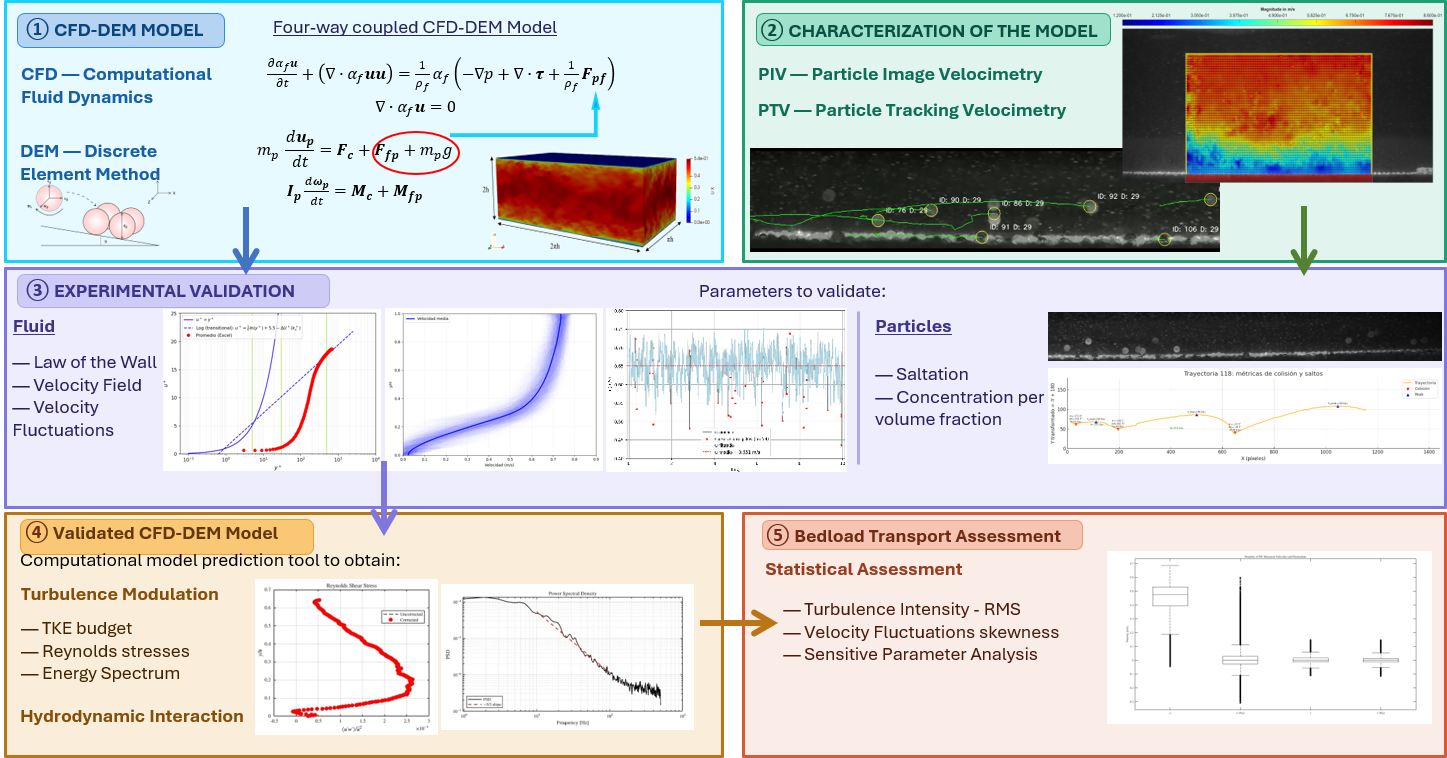
\includegraphics[width=5.99583in,height=3.14097in]{figures/image2.png}

Figure 4.1. Schematic representation from the proposed methodology.

\hypertarget{work-plan}{%
\section{Work Plan}\label{work-plan}}

El plan de trabajo de esta investigación se basa en la carta Gantt que se visualiza en la Figura 5.1, a continuación.

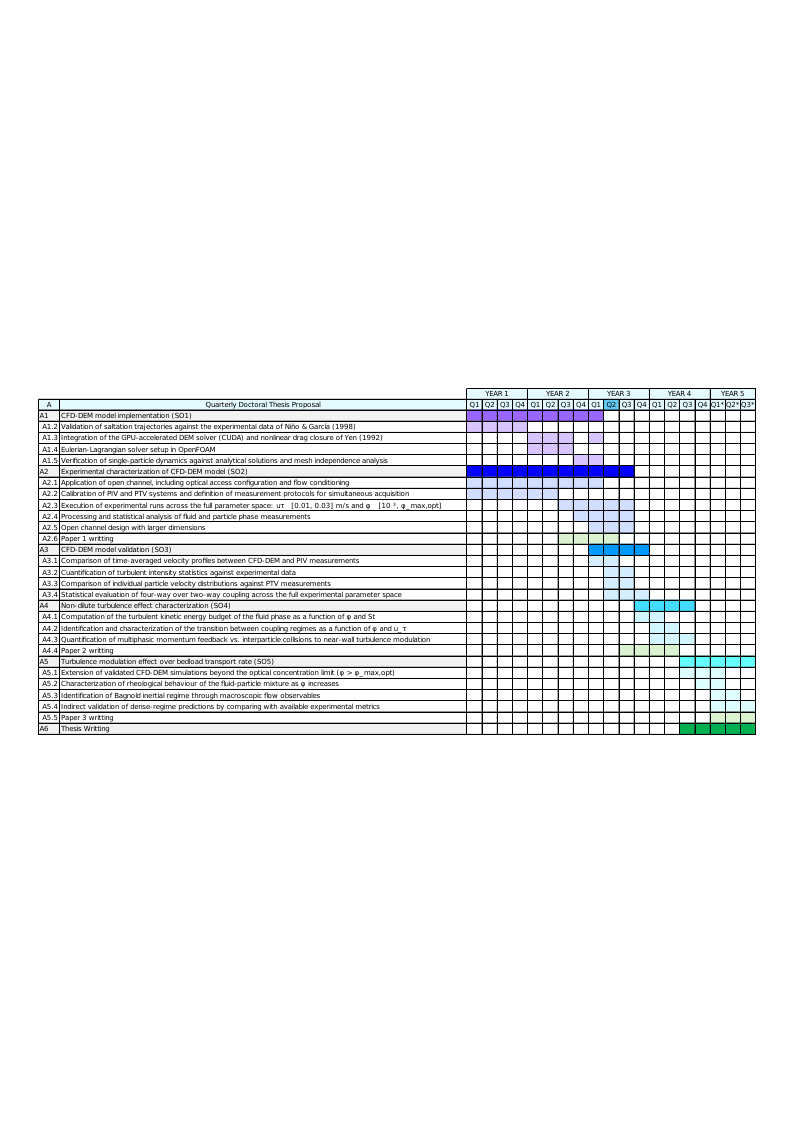
\includegraphics[width=7.55694in,height=3.64236in]{figures/image3.png}

Figure 5.1.

\hypertarget{available-resources-and-insfrastracture}{%
\subsection{Available Resources and Insfrastracture}\label{available-resources-and-insfrastracture}}

This research is funded by the National Agency for Research and Development (ANID) through the National Doctoral Scholarship. Available resources include: (1) two GPU-equipped workstations (laptop and desktop tier) for code development and small-scale runs; (2) a high-performance workstation server through the MultiphaseFlowLab research group; (3) supercomputing access through Chile's National Laboratory for High-Performance Computing (NLHPC), via the Guacolda and Leftraru Epu clusters (jointly, 91 nodes, ca.\ 9{,}956 CPU cores, InfiniBand NDR interconnect, and approximately 730 TFLOPS); and (4) the MultiphaseFlowLab's optical setup for PIV/PTV, comprising high-speed Basler cameras, precision lenses, and high-power green lasers.

\hypertarget{publishing-proposal}{%
\subsection{Publishing Proposal}\label{publishing-proposal}}

Three publications are planned, consistent with the milestones defined in the Gantt chart, also aligned with the presented objectives and methodology of this research.

P.1. ``Experimental analysis of sand transport in hydraulic channels using PIV and PTV: dilute and non-dilute concentrations across different Reynolds numbers''. \emph{Environmental fluid mechanics}.

P.2. ``Validation of a four-way coupled CFD-DEM model for predicting sand sediment transport at non-dilute concentrations using non-intrusive techniques''. \emph{Water resources research}.

P.3. ``Numerical and experimental investigation of granular bedload transport at non-dilute concentrations using a validated four-way coupled CFD-DEM model for high Reynolds number''. \emph{Journal advances in water resources}.

